\documentclass[12pt]{article}

% --- Packages ---
\usepackage[utf8]{inputenc}
\usepackage[T1]{fontenc}
\usepackage[french]{babel}
\usepackage{amsmath, amssymb}
\usepackage{geometry}
% \usepackage[draft]{graphicx}
\usepackage{tikz}
\usepackage[most]{tcolorbox}
\usepackage{multicol}
\usepackage{lmodern}
\usepackage{pgfplots}
\pgfplotsset{compat=1.18}
\usepackage{mdframed}
\usepackage{tkz-tab}
\usepackage{bm}
\usepackage{xcolor}
\usepackage{sectsty}
\usepackage[utf8]{inputenc}
\usepackage[T1]{fontenc}
\usepackage[inline]{enumitem}
\usepackage[dvipsnames]{xcolor}
\usepackage{multido}
% --- Page ---
\geometry{margin=2cm}

% Footer
\usepackage{fancyhdr}
\pagestyle{fancy}
\cfoot{\thepage}
\rfoot{\textit{G.M.}}
\renewcommand{\headrulewidth}{0pt}
\renewcommand{\footrulewidth}{0pt}

% Pour les normes : 
\newcommand*{\norme}[1]{\left\lVert\overrightarrow{#1}\right\rVert}

\usetikzlibrary{shapes.misc}

\tikzset{cross/.style={cross out, draw=black, minimum size=2*(#1-\pgflinewidth), inner sep=0pt, outer sep=0pt},
%default radius will be 1pt. 
cross/.default={4pt}}

% mettre dans le préambule, après \usepackage{xcolor}
\usepackage{sectsty} % gère facilement la couleur des titres
\setlength{\parindent}{0pt}

\sectionfont{\color{red}\Large\bfseries}     % pour \section*
\subsectionfont{\color{red}\large\bfseries\hspace{1cm}}

\begin{document}

% ============================
%   Fonctions polynômes de degré 3
% ============================

\newpage

\begin{center}
    {\LARGE \textbf{Fonctions polynômes de degré 3}}\\[4mm]
    {\large 1\up{ère} STMG - Lycée Jacques Decour}
\end{center}

\hrule
\vspace{0pt}

% ============================
%   RAPPELS : Fonctions polynômes de degré 2
% ============================

\section*{\textcolor{red}{RAPPELS : Fonctions polynômes de degré 2}}

\vspace{5pt}

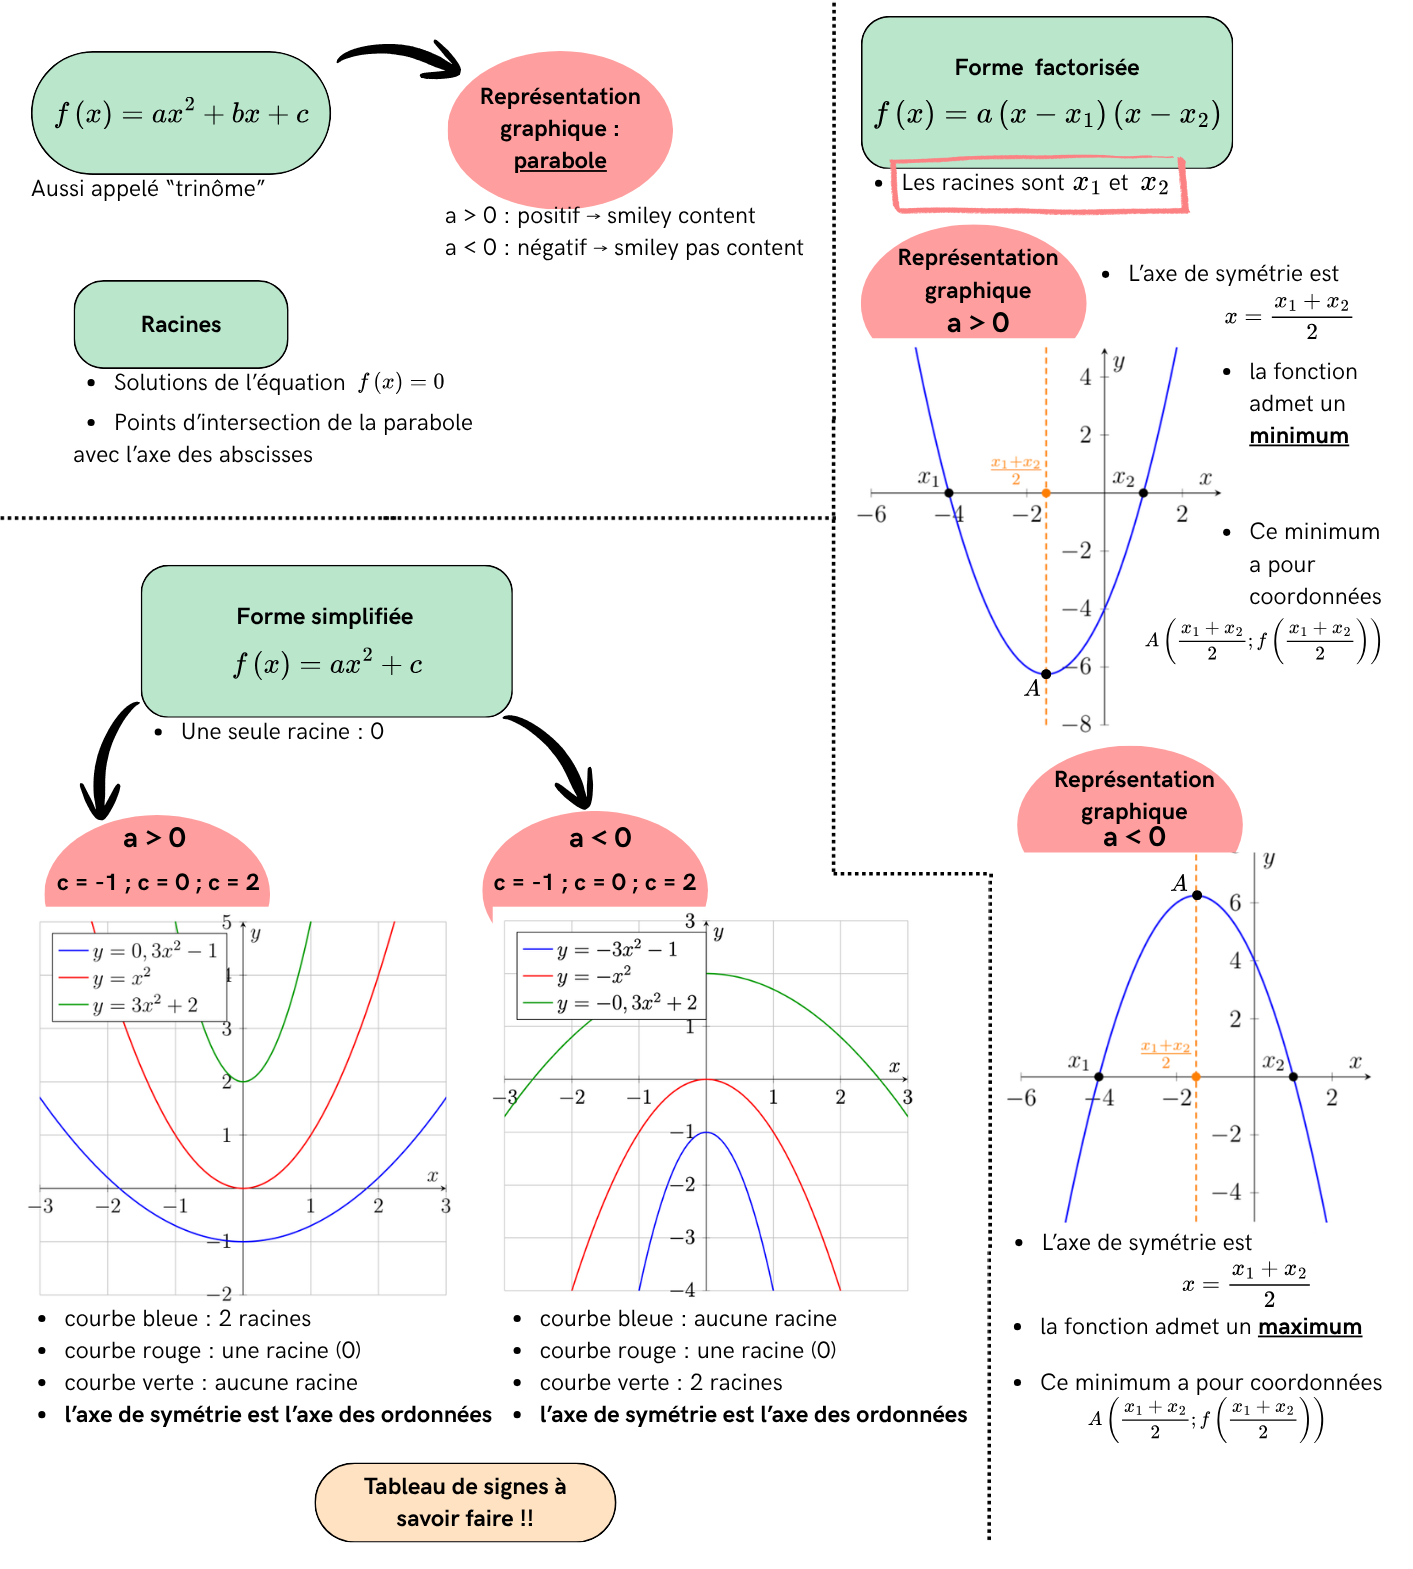
\includegraphics[width=1\textwidth]{carte mentale.png}

{\color{red}\textbf{
    Cette carte mentale ne \underline{remplace pas le cours} sur le second degré.
}}


% ========================================================
%             PARTIE 1 : Définition
% ========================================================

\section*{\textcolor{red}{PARTIE 1 : Définition}}

\vspace{5pt}

\begin{mdframed}[
    linewidth=1pt,
    roundcorner=5pt,
    linecolor=ForestGreen,
    innertopmargin=10pt,
    innerbottommargin=10pt
]
{\color{ForestGreen}
\textbf{\underline{Définition :}}}

\vspace{5pt}
On dit que $f$ est une \textbf{fonction polynôme de degré 3} lorsqu'il existe 4 réels 
$a$, $b$, $c$ et $d$, tels que $a \neq 0$ et :
\[
f(x) = ax^3 + bx^2 + cx + d
\]

\end{mdframed}

\vspace{5pt}

\underline{Exemples :}

\vspace{5pt}
Dire si ces fonctions sont des polynômes de degré 3 : 

\vspace{15pt}
$f(x) = 4x^3 + 1$ \hspace{1cm} \dotfill

\vspace{15pt}
$g(x) = -x + 4$ \hspace{1cm} \dotfill

\vspace{15pt}
$h(x) = 2x^3 - x^5 + 5x + 1$ \hspace{1cm} \dotfill

\vspace{15pt}
$m(x) = 1 + x^2 -2x^3$ \hspace{1cm} \dotfill

\vspace{15pt}
$m(x) = x^3 - 2$ \hspace{1cm} \dotfill


\vspace{20pt}


% ========================================================
%             PARTIE 2 : Fonction du type : $f(x) = ax^3 + d$
% ========================================================

\section*{\textcolor{red}{PARTIE 2 : Fonction du type : $\bm{f(x) = ax^3 + d}$}}

\vspace{5pt}

\begin{mdframed}[
    linewidth=1pt,
    roundcorner=5pt,
    linecolor=Red,
    innertopmargin=10pt,
    innerbottommargin=10pt
]
{\color{red}
\textbf{\underline{Propriété :}}

\vspace{5pt}
\begin{minipage}[t]{.45\textwidth}%
    \vspace{0pt}
    \begin{itemize}
        \item Si $a>0$, la fonction $f(x) = ax^3 + d$ est strictement \underline{croissante} sur $\mathbb{R}$.
        \vspace{10pt}
        \item Si $a<0$, la fonction $f(x) = ax^3 + d$ est strictement \underline{décroissante} sur $\mathbb{R}$.
    \end{itemize}
\end{minipage}%
\hfill
\begin{minipage}[t]{.5\textwidth}%
    \vspace{-25pt}
    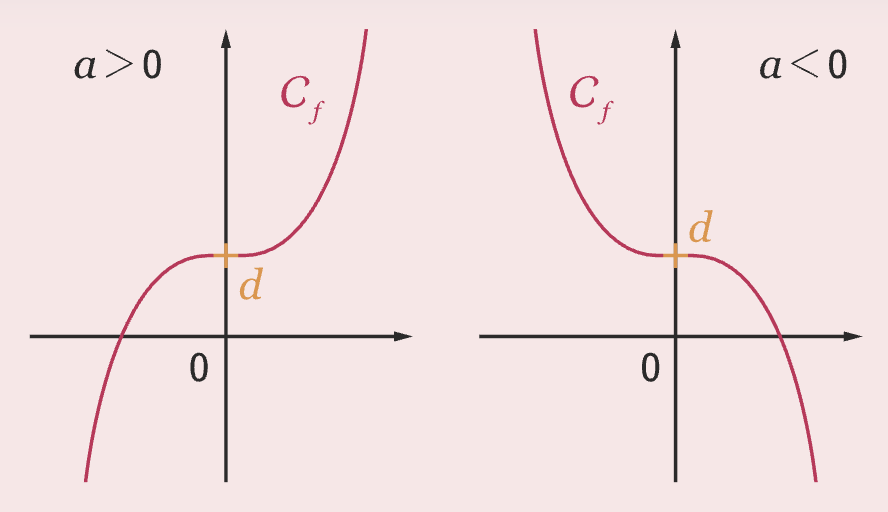
\includegraphics[width=1\textwidth]{prop11.png}
\end{minipage}%
}
\end{mdframed}

\underline{Remarque :} $d$ correspond à l'intersection de la courbe avec l'axe des ordonnées.

\vspace{5pt}
\begin{mdframed}[
    linewidth=1pt,
    roundcorner=5pt,
    linecolor=Red,
    innertopmargin=10pt,
    innerbottommargin=0pt
]
{\color{red}
\textbf{\underline{Propriété :}}

\vspace{5pt}
Soit $\alpha$ un réel. L'équation $x^3 = \alpha$ admet une unique solution sur $\mathbb{R}$ :
\[
x = \sqrt[3]{\alpha} = x^{\frac{1}{3}}
\]
}
\end{mdframed}

\vspace{5pt}
\underline{Exemple :}

\begin{itemize}
    \item L'équation $x^3 = 27$ admet une unique solution : \dotfill
    \vspace{15pt}
    \item L'équation $x^3 = -8$ admet une unique solution : \dotfill
\end{itemize}

\vspace{5pt}

\begin{mdframed}[
    linewidth=1pt,
    roundcorner=5pt,
    linecolor=RoyalBlue,
    innertopmargin=10pt,
    innerbottommargin=10pt
]
{\color{RoyalBlue}
\textbf{\underline{Exercice d'application n°1:} Résoudre une équation du type 
$\bm{x^3 = \alpha}$}}

\vspace{5pt}
Résoudre dans $\mathbb{R}$ l'équation : $2x^3 - 6 = 122$.

\vspace{0.5cm}
{\color{black!30}\dotfill}

\vspace{0.5cm}
{\color{black!30}\dotfill}

\vspace{0.5cm}
{\color{black!30}\dotfill}

\vspace{0.5cm}
{\color{black!30}\dotfill}

\vspace{20pt}

\end{mdframed}


% ========================================================
%             PARTIE 3 : Fonction du type : $f(x) = a(x - x_1)(x - x_2)(x - x_3)$
% ========================================================

\section*{\textcolor{red}{PARTIE 3 : Forme factorisée $f(x) = a(x - x_1)(x - x_2)(x - x_3)$}}

\vspace{5pt}
\underline{Exemple :}
La fonction $f$ définie par $f(x) = 5(x-4)(x-1)(x+3)$ est une fonction polynôme de degré 3 sous sa forme 
factorisée.

\vspace{5pt}
Si on développe l'expression : $f(x) = 5x^3 - 10x^2 - 55x + 60$. On obtient bien un \textbf{degré 3}.

\vspace{5pt}
\begin{mdframed}[
    linewidth=1pt,
    roundcorner=5pt,
    linecolor=ForestGreen,
    innertopmargin=10pt,
    innerbottommargin=10pt
]
{\color{ForestGreen}
\textbf{\underline{Définition :}}}

\vspace{5pt}
Les fonctions définies sur $\mathbb{R}$ par $f(x) = a(x - x_1)(x - x_2)(x - x_3)$ sont des fonctions 
polynômes de degré 3.

\vspace{5pt}
Les coefficients $a$, $x_1$, $x_2$ et $x_3$ sont des réels avec $a \neq 0$.

\end{mdframed}

\underline{Exemple :}

\vspace{5pt}
Reprenons notre exemple de tout à l'heure : 

\vspace{-10pt}
\begin{align*} % <-- observe: 'flalign*', not 'align*'
  f(x) &= 5(x-4)(x-1)(x+3) \\
  &= 5x^3 - 10x^2 - 55x + 60
\end{align*}

\vspace{5pt}
En partant de l'expression \textbf{développée}. Calculons $f(4)$, $f(1)$ et $f(-3)$.

\vspace{0.5cm}
{\color{black!30}\dotfill}

\vspace{0.5cm}
{\color{black!30}\dotfill}

\vspace{0.5cm}
{\color{black!30}\dotfill}

\vspace{0.5cm}
{\color{black!30}\dotfill}

\vspace{0.5cm}
{\color{black!30}\dotfill}

\vspace{0.5cm}
{\color{black!30}\dotfill}

\vspace{0.5cm}
{\color{black!30}\dotfill}

\vspace{20pt}

$4$, $1$ et $-3$ sont les solutions de l'équation \_\_\_\_\_\_\_\_\_\_\_\_.

\vspace{15pt}
Ce sont les \_\_\_\_\_\_\_\_\_\_\_\_\_\_\_\_\_\_\_\_\_\_\_\_.

\vspace{10pt}

\begin{mdframed}[
    linewidth=1pt,
    roundcorner=5pt,
    linecolor=Red,
    innertopmargin=10pt,
    innerbottommargin=10pt
]
{\color{red}
\textbf{\underline{Propriété :}}

\vspace{5pt}
Soit $f$ la fonction définie sur $\mathbb{R}$ par $f(x) = a(x - x_1)(x - x_2)(x - x_3)$.

\vspace{5pt}
L'équation $f(x) = 0$ possède \textbf{3 solutions} (éventuellement égales) : $x = x_1$, $x = x_2$ et $x = x_3$.

\vspace{5pt}
Ces solutions sont appelées \textbf{racines} du polynôme $a(x - x_1)(x - x_2)(x - x_3)$.
}
\end{mdframed}


\vspace{5pt}
\underline{Exemple :}

\vspace{5pt}
\begin{minipage}[t]{.45\textwidth}%
    \vspace{0pt}
    On considère la fonction : 
    
    \vspace{5pt}
    $f(x) = \dfrac{1}{100}(x+5)(x+2)(x-4)$
    
    \vspace{5pt}
    définie sur $\mathbb{R}$ et représentée 
    ci-contre.

\end{minipage}%
\hfill
\begin{minipage}[t]{.5\textwidth}%
    \vspace{-20pt}
    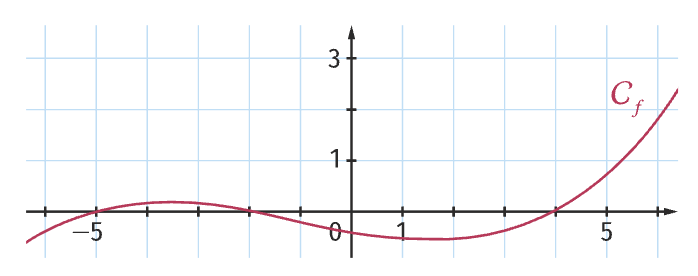
\includegraphics[width=1\textwidth]{exemple1.png}
\end{minipage}%

\vspace{10pt}
Les racines de ce polynôme sont : \vspace{0.5cm}
{\color{black!30}\dotfill}


\vspace{10pt}

{\color{RedOrange}\textbf{\underline{Méthode :} Étudier le signe d'un polynôme de degré 3}}

\vspace{5pt}
Étudier le signe de la fonction polynôme :
\[
f(x) = 2(x+1)(x-2)(x-5)
\]

$2$ étant un nombre \textbf{positif}, le signe de $2(x+1)(x-2)(x-5)$ dépend du signe de chacun des 

\vspace{15pt}
facteurs :
{\color{black!30}\dotfill}

\vspace{20pt}

\begin{mdframed}[
    linewidth=1pt,
    roundcorner=5pt,
    linecolor=Red,
    innertopmargin=10pt,
    innerbottommargin=10pt
]
{\color{red}
\textbf{\underline{RAPPEL :} Comment étudier le signe d'une fonction affine de la forme $ax + b$}}

\vspace{5pt}
Exemple : $f(x) = -2x+3$.

\vspace{5pt}
On commence par trouver la valeur où ça change de signe en résolvant l'équation :

\newpage
Pour remplir les signes dans le tableau de signes, on applique la propriété suivante :
{\color{red}
\begin{itemize}
    \item $a>0$ alors d'abord un signe $-$ puis un signe $+$
    \item $a<0$ alors d'abord un signe $+$ puis un signe $-$
\end{itemize}
}
On construit alors le tableau de signe suivant : 

\[
\begin{tikzpicture}
   \tkzTabInit[lgt = 2.5]{$x$ / 1 , $f(x)$ / 1}
   {$-\infty$, , $+\infty$}
   \tkzTabLine{, , ,}
\end{tikzpicture}
\]

\end{mdframed}

\vspace{5pt}
Étudions le signe de chacun des facteurs : 

\vspace{0.5cm}
{\color{black!30}\dotfill}

\vspace{0.5cm}
{\color{black!30}\dotfill}

\vspace{0.5cm}
{\color{black!30}\dotfill}

\vspace{0.5cm}
{\color{black!30}\dotfill}

\vspace{20pt}
Et on présente le tout sous la forme d'un grand tableau de signes : 

\vspace{10pt}
\[
\begin{tikzpicture}
   \tkzTabInit[lgt = 2.5]{$x$ / 1 , $x+1$ / 1, $x-2$ / 1, $x-5$ / 1, $f(x)$ / 1}
   {$-\infty$, , , , $+\infty$}
   \tkzTabLine{, , , , , , }
   \tkzTabLine{, , , , , , }
   \tkzTabLine{, , , , , , }
\end{tikzpicture}
\]

\vspace{10pt}
On en déduit que $f(x) \leq 0$ sur \_\_\_\_\_\_\_\_\_\_\_\_\_\_\_\_\_\_\_\_\_\_\_\_.

\vspace{20pt}
Et que $f(x) \geq 0$ sur \_\_\_\_\_\_\_\_\_\_\_\_\_\_\_\_\_\_\_\_\_\_\_\_.

\vspace{20pt}
\hspace{6cm}\underline{Voici un schéma explicatif :}

\vspace{-60pt}
\hspace{12cm}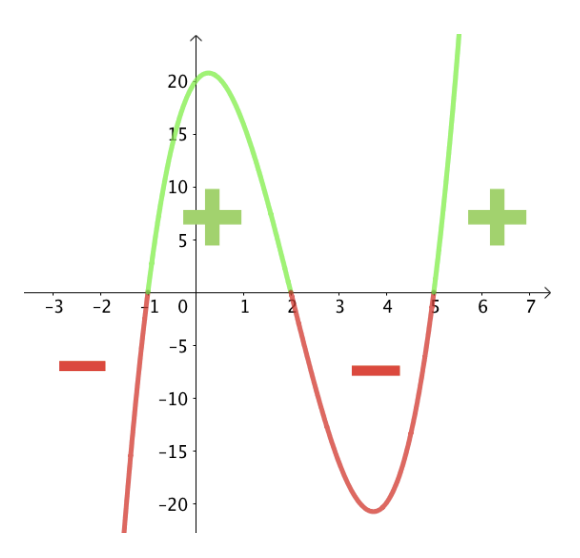
\includegraphics[width=0.3\textwidth]{schema1.png}




\end{document}
